\documentclass[10pt, compress]{beamer}

\usetheme{m}

\usepackage{booktabs}
\usepackage[scale=2]{ccicons}
\usepackage{minted}

\usemintedstyle{trac}

\usepackage{tikz}
\usepackage{tikz-qtree}
\usetikzlibrary{matrix,backgrounds, decorations.pathreplacing, automata, arrows}

\tikzset{onslide/.code args={<#1>#2}{%
  \only<#1>{\pgfkeysalso{#2}} % \pgfkeysalso doesn't change the path
}}
\tikzset{
  invisible/.style={opacity=0},
  visible on/.style={alt={#1{}{invisible}}},
  alt/.code args={<#1>#2#3}{%
    \alt<#1>{\pgfkeysalso{#2}}{\pgfkeysalso{#3}} % \pgfkeysalso doesn't change the path
  },
  blink/.style={onslide={<#1> mLightBrown}},
  appear/.style={visible on=<#1->, blink=#1}
}

\newcommand{\tdots}{\,.\,.\,} % in place of \ldots
\newcommand{\E}{\Sigma}
\newcommand{\Oh}{\mathcal{O}}
\newcommand{\cS}{\mathcal{S}}


\title{Algoritmo de Aho-Corasick}
\subtitle{Yan Soares Couto}
\date{2017}
\author{Orientadora: Cristina Gomes Fernandes}
\institute{Instituto de Matemática e Estatística}


\begin{document}

\maketitle

\begin{frame}[fragile]
  \frametitle{definição}

String~$S[1\tdots|S|]$: vetor em que cada elemento é de um alfabeto~$\E$ finito.

Em geral,~$\E = \{\text{a}, \text{b}, \ldots, \text{z}\}$.

\pause
\begin{center}
{\huge ``abracadabra''}
\end{center}

Substring de~$S$: subvetor de~$S$, por exemplo, {\large``cadab''}.

\end{frame}

\section{KMP}

\begin{frame}[fragile]
\frametitle{Bordas}

Borda de uma string: Maior prefixo que é também sufixo da string.
\pause

\vfill
\begin{center}
{\large abracadabra} $\Rightarrow$ {\large abra}

{\large casa} $\Rightarrow$ {\large $\varepsilon$}

{\large botobot} $\Rightarrow$ {\large bot}
\end{center}
\vfill

\end{frame}

\begin{frame}[fragile]
\frametitle{Bordas}
KMP calcula o tamanho da borda de todo prefixo da string.

\begin{center}
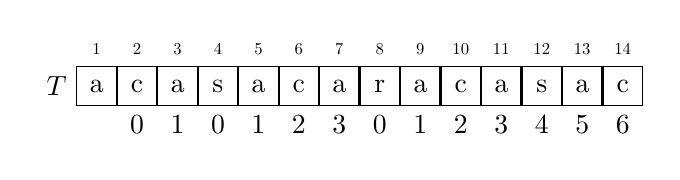
\begin{tikzpicture}
\matrix[matrix of nodes, nodes in empty cells,
row 1/.style={nodes={scale=.6, minimum size = 5mm}},
row 2/.style={nodes={draw, minimum size = 5mm,anchor=center}},
row 2 column 1/.style={nodes={draw=none}}
] (array) {
    & 1 & 2 & 3 & 4 & 5 & 6 & 7 & 8 & 9 & 10 & 11 & 12 & 13 & 14 \\
$T$ & a & c & a & s & a & c & a & r & a & c & a & s & a & c \\
    &   & 0 & 1 & 0 & 1 & 2 & 3 & 0 & 1 & 2 & 3 & 4 & 5 & 6 \\
};

\end{tikzpicture}
\end{center}

\end{frame}

\section{Tries}

\begin{frame}[fragile]
\frametitle{Definição}

\textbf{Trie}: árvore enraizada que armazena um conjunto de strings.

Strings são representadas como caminhos a partir da raiz.

\end{frame}

\begin{frame}[fragile]
\frametitle{Construção}

\begin{center}
\begin{tikzpicture}[sibling distance=25pt]
\Tree [.{}
\edge[appear=2]; [.\node[appear=2,blink=6]{m}; \edge[appear=3]; [.\node[appear=3,blink=7]{a}; \edge[appear=8]; [.\node[appear=8]{m}; \edge[appear=9]; [.\node[appear=9]{a}; \edge[appear=10]; [.\node[appear=10]{t}; \edge[appear=11]; \node[appear=11,draw]{a}; ] ] ] \edge[appear=4]; [.\node[appear=4]{t};  \edge[appear=5]; \node[appear=5, draw]{a}; ] ] ]
%
%
\edge[appear=12]; [.\node[appear=12,blink=16, blink=18]{o}; \edge[appear=13]; [.\node[appear=13,onslide={<17-> draw}, blink=17]{i}; \edge[appear=14]; [.\node[appear=14]{t}; \edge[appear=15]; \node[appear=15,draw]{o}; ] ] \edge[appear=19]; [.\node[appear=19]{m}; \edge[appear=20]; [.\node[appear=20]{a}; \edge[appear=21]; \node[appear=21,draw]{r}; ] ] ]
]
\end{tikzpicture}

Adicionando \only<1-5>{\large ``mata''.} \only<6-11>{\large ``mamata''.} \only<12-15>{\large ``oito''.} \only<16-17>{\large ``oi''.} \only<18-22>{\large ``omar''.}
\end{center}

\end{frame}

\begin{frame}[fragile]
\frametitle{Usos}

Construir uma trie para~$\cS = \{S_1, \ldots, S_k\}$ consome tempo~$\Oh(\sum\limits_{i=1}^k{|S_i|})$.

Com esta trie, podemos realizar:
\begin{description}
\item [\textsc{Contains}$(S)$] Determina se~$S \in \cS$.
\item [\textsc{LCP}$(S)$] Determina o maior prefixo comum de~$S$ com alguma string de~$\cS$.
\end{description}

Consumo de tempo:~$\Oh(|S|)$.


\end{frame}

\section{Aho-Corasick}

\begin{frame}[fragile]
\frametitle{Introdução}

\alert{Problema:} Determine todas as ocorrências de todas as strings de~$\cS = \{S_1, \ldots, S_k\}$ em~$T$.
\vspace{2ex}

\pause

Para cada sufixo~$T[i\tdots |T|]$, usando uma trie, determinamos as strings de~$\cS$ que ocorrem \textbf{no início} de~$T[i\tdots |T|]$.

Isso leva tempo~$\Oh(|T|^2)$.

\end{frame}

\begin{frame}[fragile]
\frametitle{Links de falha}

No KMP: função prefixo guarda, para cada~$i$, o comprimento do maior prefixo de~$T$ que é sufixo próprio de~$T[1\tdots i]$.

\begin{center}
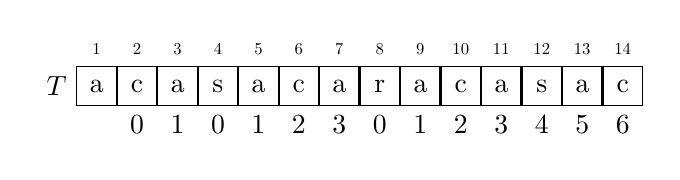
\begin{tikzpicture}
\matrix[matrix of nodes, nodes in empty cells,
row 1/.style={nodes={scale=.6, minimum size = 5mm}},
row 2/.style={nodes={draw, minimum size = 5mm,anchor=center}},
row 2 column 1/.style={nodes={draw=none}}
] (array) {
    & 1 & 2 & 3 & 4 & 5 & 6 & 7 & 8 & 9 & 10 & 11 & 12 & 13 & 14 \\
$T$ & a & c & a & s & a & c & a & r & a & c & a & s & a & c \\
    &   & 0 & 1 & 0 & 1 & 2 & 3 & 0 & 1 & 2 & 3 & 4 & 5 & 6 \\
};

\end{tikzpicture}
\end{center}

\pause
Em Tries: para cada nó~$v$, guarda o nó mais profundo cuja string seja um sufixo próprio da string de~$v$.

\begin{center}
\emph{\huge link de falha}
\end{center}

%Ou seja, queremos para cada prefixo~$S_1[1\tdots i]$ de \textbf{alguma} string de~$\cS$, queremos encontrar o maior prefixo~$S_2[1\tdots j]$ de \textbf{alguma} (possivelmente outra) string de~$\cS$ tal que~$S_2[1\tdots j]$ seja sufixo próprio de~$S_1[1\tdots i]$.

\end{frame}

\begin{frame}[fragile]
\frametitle{Links de falha}

Para cada nó~$v$, guardar o nó mais profundo cuja string seja um \alert{sufixo próprio} da string de~$v$.

\begin{center}
\centering
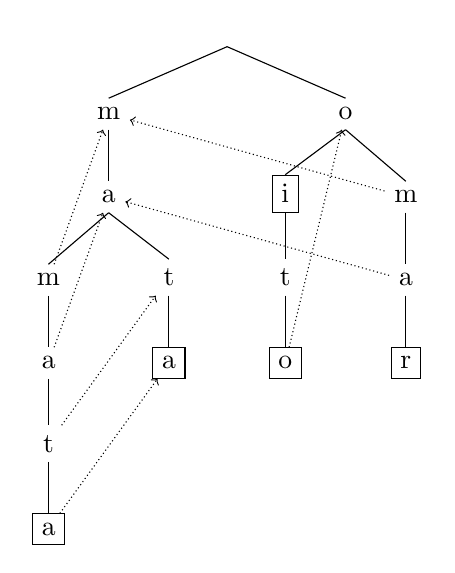
\begin{tikzpicture}[sibling distance=30pt]
\Tree [.{}
[.\node(m){m}; [.\node(ma){a}; [.\node(mam){m}; [.\node(mama){a}; [.\node(mamat){t}; \node[draw](mamata){a}; ] ] ] [.\node(mat){t}; \node[draw](mata){a}; ] ] ]
[.\node(o){o}; [.\node[draw](oi){i}; [.\node(oit){t}; \node[draw](oito){o}; ] ] [.\node(om){m}; [.\node(oma){a}; \node[draw](omar){r}; ] ] ]
]
%\draw[semithick,->] (t)..controls +(south west:5) and +(south:5)..(wh);
\draw[densely dotted,->] (mamata) -- (mata);
\draw[densely dotted,->] (mamat) -- (mat);
\draw[densely dotted,->] (mama) -- (ma);
\draw[densely dotted,->] (mam) -- (m);
\draw[densely dotted,->] (oito) -- (o);
\draw[densely dotted,->] (oma) -- (ma);
\draw[densely dotted,->] (om) -- (m);
\end{tikzpicture}
\end{center}

\end{frame}

\begin{frame}[fragile]
\frametitle{Algoritmo}

Para cada prefixo~$T[1\tdots i]$, determinar o maior prefixo~$S[1\tdots j]$ de alguma string de~$\cS$ que é sufixo de~$T[1\tdots i]$.

\end{frame}

\begin{frame}[fragile]
\frametitle{Algoritmo}

\begin{center}

\begin{tikzpicture}
\matrix[matrix of nodes, nodes in empty cells,
row 1/.style={nodes={scale=.6, minimum size = 5mm}},
row 2/.style={nodes={draw, minimum size = 5mm,anchor=center}},
row 2 column 1/.style={nodes={draw=none}}
] (array) {
    & \node[onslide={<2> mLightBrown}]{1}; & \node[onslide={<3> mLightBrown}]{2}; & \node[onslide={<4> mLightBrown}]{3}; & \node[onslide={<5> mLightBrown}]{4}; & \node[onslide={<6> mLightBrown}]{5}; & \node[onslide={<7> mLightBrown}]{6}; & \node[onslide={<8> mLightBrown}]{7}; & \node[onslide={<9> mLightBrown}]{8}; \\
$T$ & o & m & a & m & a & t & a & m \\
};

\end{tikzpicture}


\begin{tikzpicture}[sibling distance=30pt]
\Tree [.{}
[.\node(m)[onslide={<9> mLightBrown}]{m$\onslide<9->{_8}$}; [.\node(ma){a}; [.\node(mam)[onslide={<5> mLightBrown}]{m$\onslide<5->{_4}$}; [.\node(mama)[onslide={<6> mLightBrown}]{a$\onslide<6->{_5}$}; [.\node(mamat)[onslide={<7> mLightBrown}]{t$\onslide<7->{_6}$}; \node[draw](mamata)[onslide={<8> mLightBrown}]{a$\onslide<8->{_7}$}; ] ] ] [.\node(mat){t}; \node[draw](mata){a}; ] ] ]
[.\node(o)[onslide={<2> mLightBrown}]{o$\onslide<2->{_1}$}; [.\node[draw](oi){i}; [.\node(oit){t}; \node[draw](oito){o}; ] ] [.\node(om)[onslide={<3> mLightBrown}]{m$\onslide<3->{_2}$}; [.\node(oma)[onslide={<4> mLightBrown}]{a$\onslide<4->{_3}$}; \node[draw](omar){r}; ] ] ]
]
%\draw[semithick,->] (t)..controls +(south west:5) and +(south:5)..(wh);
\draw[densely dotted,->] (mamata) -- (mata);
\draw[densely dotted,->] (mamat) -- (mat);
\draw[densely dotted,->] (mama) -- (ma);
\draw[densely dotted,->] (mam) -- (m);
\draw[densely dotted,->] (oito) -- (o);
\draw[densely dotted,->] (oma) -- (ma);
\draw[densely dotted,->] (om) -- (m);
\end{tikzpicture}
\end{center}


\end{frame}

\begin{frame}[fragile]
\frametitle{Considerações finais}

Uma string de~$\cS$ pode ser sufixo \alert{próprio} de~$S[1\tdots j]$!

\textbf{link de ocorrência} de $v$: vértice que representa a maior string de~$\cS$ que é sufixo próprio da string de~$v$.

\pause

O algoritmo pode ser implementado em tempo~$\Oh(\sum\limits_{i=1}^k{|S_i||\E|} + |T| + x)$, onde~$x$ é o número de ocorrências.

\end{frame}

\plain{}{\alert{Perguntas?}}

\end{document}
